\documentclass[11pt]{article}
\usepackage{vmargin}
\usepackage{graphicx}
\usepackage{amssymb}
\usepackage{epstopdf}
\usepackage{epsfig}
\usepackage{alltt}
\usepackage{bm}
\usepackage{amsmath}
\usepackage{color}
\usepackage{drawstack}
\usepackage{tikz}
\usetikzlibrary{shapes,arrows,shapes.multipart,backgrounds,calc,positioning}
\DeclareGraphicsRule{.tif}{png}{.png}{`convert #1 `dirname #1`/`basename #1 .tif`.png}
\newcommand{\sbt}{\,\begin{picture}(-1,1)(-1,-3)\circle*{3}\end{picture}\ }
\newcommand{\ith}{$i^{th}$}

\textwidth = 6.5 in
\textheight = 9 in
\oddsidemargin = 0.5 in
\evensidemargin = 0.5 in
\parskip = 0.2in
\parindent = 0.0in

\newcommand*{\tabbox}[2][t]{%
    \vspace{0pt}\parbox[#1][3.7\baselineskip]{1cm}{\strut#2\strut}}
    
\title{CS652 Smalltalk VM Operational Semantics}
\author{Terence Parr}
\begin{document}
\maketitle

\def\arraystretch{1.25}

\begin{figure}
\begin{center}
\begin{tabular}{l p{8cm}}
$T \bowtie x$ & Resolve $x$ in scope $T$ \\

$o \in \text{\tt X}$ & $o$ is instance of $X$\\

${\bf v} \in \text{\tt STObject}$ & a single object \\

${\bm l_i} \in \text{\tt STObject}$ & the \ith argument or local variable object \\

$o_{class} \in \text{\tt\small STMetaClassObject}$ & Metaclass (type) of object $o$\\

$o_{class_{class}}=o_{class}$ &  A metaclass object is its own type\\

$o_{superclass} \in \text{\tt\small STMetaClassObject}$ & Superclass (type) of object $o$\\

$o_{field_i}$ & The \ith field of object $o$ \\

$f_{literal_i}$ & The \ith literal of method $f$ \\

$f^{block_i}_s \in \text{\tt\small BlockDescriptor}$ & The \ith block of method $f$ associated with instance self=$s$\\

$f^{block_i}_s[\_,\_,\_] \in \text{\tt\small BlockContext}$ & The \ith block of method $f$ invoked with self=$s$\\

$f^{block_i}_s[\_,\_,\_]^d \in \text{\tt\small BlockContext}$ & The \ith block of method $f$ invoked with self=$s$ and having depth $d$ counting from zero at the method block; e.g., {\tt f [|x| [|y|]]} has a method block at depth 0 with {\tt x} and a nested block at depth 1 with {\tt y} \\

$\gamma \in \text{\tt\small MethodContext}^*$ & Stack of method invocations growing to the right\\

$\delta \in \text{\tt\small STObject}^*$ &  Operand stack of objects growing to the right\\

$\mathbb{S}$ & The state of the VM system dictionary\\

$(\mathbb{S},\gamma)$ & VM state is the system dictionary and a method invocation stack with zero or more elements\\

$(\mathbb{S}, \gamma) \Rightarrow (\mathbb{S}', \gamma')$ & VM state transition\\

$(\mathbb{S}, \gamma) \Rightarrow^* (\mathbb{S}', \gamma')$ & Zero-or-more state transitions\\

$f_s[ip,l_0,..l_{n-1},\delta]$ & Method invocation context that derived from sending message $f$ to receiver $s$ (self);  $f \in \text{\tt\small MethodContext}$; $l_i$ is local variable or argument, indexed from 0 and arguments first; $\delta$ is the operand stack; $f$ {\em can also represent a nested code block not just a  method} \\

$f[ip,l_0,..l_{n-1},\delta]$ & Same as previous but the receiver is unknown or irrelevant \\

$f[ip,\_,\_]$ & A method invitation context with ``don't care'' for locals and operand stack\\

\end{tabular}
\end{center}
\vspace{-10pt}
\caption{\small Smalltalk VM Bytecode Specification Notation}
\label{acfg}
\end{figure} 

\def\arraystretch{1.25}

%------------VM TRANSITIONS---------------------

\begin{figure}
\begin{center}
\begin{tabular}[t]{r | l}
{\bf Bytecode Instruction} & {\bf Transition} \\
\hline
{\em initial state} &
\begin{minipage}[t]{.7\linewidth}
$state_0 = (\mathbb{S}[\text{\tt Transcript}], \text{\tt main}_{m}[0,\epsilon,\epsilon])$\\
for $m \in \text{\tt MainClass}$; program terminates if $\exists~ state_0 \Rightarrow^* (\mathbb{S'}, \epsilon)$ 
\end{minipage}\\
\hline
{\tt nil}  & $(\mathbb{S}, \gamma f[ip,\_,\delta]) ~\Rightarrow~ (\mathbb{S}, \gamma f[ip+1,\_,\delta\, \text{\tt nil}])$\\

{\tt self} & $(\mathbb{S},\gamma f_s[ip,\_,\delta]) ~\Rightarrow~ (\mathbb{S},\gamma f_s[ip+1,\_,\delta \,s])$ \\

{\tt true} & $(\mathbb{S},\gamma f[ip,\_,\delta]) ~\Rightarrow~ (\mathbb{S},\gamma f[ip+1,\_,\delta \,\text{\tt true}])$\\

{\tt false} & $(\mathbb{S},\gamma f[ip,\_,\delta]) ~\Rightarrow~ (\mathbb{S},\gamma f[ip+1,\_,\delta \,\text{\tt false}])$\\

{\tt push\_char} $c$ & $(\mathbb{S},\gamma f[ip,\_,\delta]) ~\Rightarrow~ (\mathbb{S},\gamma f[ip+3,\_,\delta \,c])$]\\

{\tt push\_int} $i$ & $(\mathbb{S},\gamma f[ip,\_,\delta]) ~\Rightarrow~ (\mathbb{S},\gamma f[ip+5,\_,\delta \,i])$\\

{\tt push\_float} $i$ & $(\mathbb{S},\gamma f[ip,\_,\delta]) ~\Rightarrow~ (\mathbb{S},\gamma f[ip+5,\_,\delta \, \text{\em intBitsToFloat}(i)])$\\

{\tt push\_field} $i$ & $(\mathbb{S},\gamma f_s[ip,\_,\delta]) ~\Rightarrow~ (\mathbb{S}, \gamma f_s[ip+3,\_,\delta \,s_{field_i}])$ \\

{\tt push\_local} $0, i$ & $(\mathbb{S},\gamma f[ip,\cdots l_i \cdots,\delta]) ~\Rightarrow~ (\mathbb{S},\gamma f[ip+5,\cdots l_i\cdots,\delta \,l_i])$\\

{\tt push\_local} $n > 0, i$ &
\begin{minipage}[t]{.78\linewidth}
$(\mathbb{S},\gamma g^{block}[\_,\cdots {\bm l_i} \cdots,\_]^{d-n} \,\cdots\, g^{block'}[ip,\_,\_]^{d-1}\,\cdots\, g^{block''}[ip,\_,\delta]^{d}) ~\Rightarrow\\
(\mathbb{S},\gamma\, \cdots \,g^{block''}[ip+5,\_,\delta {\bm l_i}]^{d})$
\end{minipage} \\

{\tt push\_literal} $i$ & $(\mathbb{S},\gamma f[ip,\_,\delta]) ~\Rightarrow~ (\mathbb{S},\gamma f[ip+3,\_,\delta \,f_{literal_i}])$ \\

{\tt push\_global} $i$  & $(\mathbb{S},\gamma f[ip,\_,\delta]) ~\Rightarrow~ (\mathbb{S},\gamma f[ip+3,\_,\delta \,\mathbb{S}[f_{literal_i}]])$ \\

{\tt push\_array} $n$  &  $(\mathbb{S},\gamma f[ip,\_,\delta\,a_1..a_n]) ~\Rightarrow~ (\mathbb{S}, \gamma f[ip+3,\_,\delta A])$ where $A = Array(a_1..a_n)$ \\

{\tt store\_field} $i$ & $(\mathbb{S}, \gamma f_s[ip,\_,\delta \,{\bf v}]) ~\Rightarrow~ (\mathbb{S}[s_{field_i} = {\bf v}],\gamma f_s[ip+3,\_,\delta\, {\bf v}])$ \\

{\tt store\_local} $n,i$ & $(\mathbb{S},\gamma f[ip, \cdots l_i\cdots,\delta \,{\bf v}]) ~\Rightarrow~ (\mathbb{S},\gamma f[ip+5,\cdots l_{i-1} {\bf v} \,l_{i+1}\cdots,\delta \,{\bf v}])$ \\

{\tt pop} & $(\mathbb{S},\gamma f[ip,\_,\delta \,{\bf v}]) ~\Rightarrow~ (\mathbb{S},\gamma f[ip+1,\_,\delta])$\\
\hline

{\tt send} $n,i$ & 
\begin{minipage}[c]{.78\linewidth}
$(\mathbb{S},\gamma f[ip,\_,\delta \,r\, p_1 .. p_{n}]) \Rightarrow 
(\mathbb{S},\gamma f[ip+5,\_,\delta] ~(r_{class}\,{\small \bowtie} \,f_{literal_i})_r[0,p_1 .. p_{n},\epsilon])$
\end{minipage}\\

{\tt send\_super} $n,i$ & 
\begin{minipage}[c]{.78\linewidth}
$(\mathbb{S},\gamma f[ip,\_,\delta \,r\, p_1 .. p_{n}]) \Rightarrow 
(\mathbb{S},\gamma f[ip+5,\_,\delta] ~(r_{superclass}\,{\small \bowtie} \,f_{literal_i})_r[0,p_1 .. p_{n},\epsilon])$
\end{minipage}\\

{\tt block} $i$  & $(\mathbb{S},\gamma f[ip,\_,\delta]) ~\Rightarrow~ (\mathbb{S},\gamma f[ip+3,\_,\delta \,f^{block_i}_s])$\\

{\tt block\_return} &  $(\mathbb{S},\gamma f[ip,\_,\delta]~g^{block}[\_,\_,\delta' \,{\bf v}]) ~\Rightarrow~ (\mathbb{S},\gamma f[ip,\_,\delta \,{\bf v}])$\\

({\em method local}) ~~{\tt return} & $(\mathbb{S},\gamma f[ip,\_,\delta] ~g[\_,\_,\delta' \,{\bf v}]) ~\Rightarrow~ (\mathbb{S},\gamma f[ip,\_,\delta \,{\bf v}])$\\

({\em method nonlocal}) ~~{\tt return} & $(\mathbb{S},\gamma f[ip,\_,\delta] ~g_s[\_,\_,\_]~ \cdots ~h[\_,\_,\_] ~ g^{block}_s[\_,\_,\delta' \,{\bf v}]) ~\Rightarrow~ (\mathbb{S},\gamma f[ip,\_,\delta \,{\bf v}])$\\

\hline

{\tt dbg} $i, loc$ &
\begin{minipage}[t]{.76\linewidth}
$(\mathbb{S},\gamma f[ip,\_,\_])\Rightarrow
 (\mathbb{S}[\text{\it file}\text{=}f_{literal_i}, \text{\it line}\text{=}loc[31\text{:}8], \text{\it col}\text{=}loc[7\text{:}0]],\gamma f[ip+7,\_,\_])$ \\
Set VM current filename to $f_{literal_i}$ and split $loc$ into char position (indexed from 0) from lower 8 bits and line number  from the upper 24 bits.
\end{minipage}\\
\end{tabular}
\end{center}
\vspace{-10pt}
\caption{Smalltalk VM State Transition Rules}
\label{default}
\end{figure}%

%------------BYTECODE DEFS---------------------

\begin{figure}
\begin{center}
\begin{tabular}[t]{r | l}
{\bf Bytecode Instruction} & {\bf Description} \\
\hline
{\tt nil}  & \begin{minipage}[t]{.76\linewidth}Push {\tt nil} onto the operand stack of the {\em current block or method context}.\end{minipage} \\

{\tt self} & \begin{minipage}[t]{.76\linewidth}Push {\tt self}, the current method's receiver object, onto the operand stack\end{minipage} \\

{\tt true} & \begin{minipage}[t]{.76\linewidth}Push {\tt true} onto the operand stack\end{minipage} \\

{\tt false} & \begin{minipage}[t]{.76\linewidth}Push {\tt false} onto the operand stack\end{minipage} \\

{\tt push\_char} $c$ & \begin{minipage}[t]{.76\linewidth}Push character $c$ onto the operand stack\end{minipage} \\

{\tt push\_int} $i$ & \begin{minipage}[t]{.76\linewidth} Push integer $i$ onto the operand stack\end{minipage} \\ 

{\tt push\_float} $f$ & \begin{minipage}[t]{.76\linewidth} Push floating-point $f$\end{minipage} \\

{\tt push\_field} $i$ & \begin{minipage}[t]{.76\linewidth} Push field at index $i$ of {\tt self}\end{minipage} \\

{\tt push\_local} $0, i$ & \begin{minipage}[t]{.76\linewidth} Push the local variable or method argument at index $i$ of the current context onto the operand stack of the current context\end{minipage} \\

{\tt push\_local} $n > 0, i$ & \begin{minipage}[t]{.76\linewidth}Push the local variable or method argument at index $i$ of the  context $n$ callers above (stack growing downwards) onto the operand stack of the current context\end{minipage} \\

{\tt push\_literal} $i$ & \begin{minipage}[t]{.76\linewidth} Push string literal at literal index $i$ onto the stack\end{minipage} \\

{\tt push\_global} $i$  & \begin{minipage}[t]{.76\linewidth} Look up string at literal index $i$ in the global scope and push that object onto the operand stack of the current context. This is used to look up class definition objects primarily as in {\tt Array new}. \end{minipage} \\

{\tt push\_array} $n$  & \begin{minipage}[t]{.76\linewidth}Pop $n$ items from the operand stack, create an array of them, push the array back to the operand stack\end{minipage} \\

{\tt store\_field} $i$ & \begin{minipage}[t]{.76\linewidth}Store the top of the operand stack into field $i$ of {\tt self}; does {\em not} pop the operand stack\end{minipage} \\

{\tt store\_local} $n,i$ & \begin{minipage}[t]{.76\linewidth}Store the top of the operand stack into local $i$ of the current context; does {\em not} pop the operand stack\end{minipage} \\

{\tt pop} & \begin{minipage}[t]{.76\linewidth}Pop the top of the operand stack off\end{minipage} \\
\hline

{\tt send} $n,i$ & \begin{minipage}[t]{.76\linewidth} Send message with $n$ arguments to method identified by string literal $i$ (in current context). The receiver of the message send is pushed on the stack before the arguments so this instruction pops $n+1$ items from the operand stack. The method is looked up in the class of the receiver object\end{minipage} \\

{\tt send\_super} $n,i$ & \begin{minipage}[t]{.76\linewidth}Same as {\tt send} except that the method is looked up in the superclass of {\tt self}'s class. The receiver is always {\tt self}\end{minipage} \\

{\tt block} $i$  & \begin{minipage}[t]{.76\linewidth}Push the block descriptor identified by index $i$ onto the operand stack of the current context\end{minipage} \\

{\tt block\_return} & \begin{minipage}[t]{.76\linewidth} Pop the return value on the top of the operand stack of the current context and push it on the operand stack of the caller's context. Pop the context stack.\end{minipage} \\

({\em method local}) ~~{\tt return} & \begin{minipage}[t]{.76\linewidth}Pop the top of the operand stack of the current context and push it on the operand stack of the caller's context. Pop the context stack.\end{minipage} \\

({\em method nonlocal}) ~~{\tt return} & \begin{minipage}[t]{.76\linewidth}Pop the top of the operand stack of the current context, unwind the call stack until the *enclosing method* of the current block, pop to the caller, push the return value onto the operand stack\end{minipage} \\

\hline

{\tt dbg} $i, loc$ & 
\begin{minipage}[t]{.76\linewidth}
Set VM current filename to $f_{literal_i}$ and split $loc$ into char position (indexed from 0) from lower 8 bits and line number  from the upper 24 bits. $\text{\it line}\text{=}loc[31\text{:}8], \text{\it col}\text{=}loc[7\text{:}0]]$
\end{minipage}\\

\end{tabular}
\end{center}
\vspace{-10pt}
\caption{Smalltalk VM Bytecode}
\label{default}
\end{figure}%


%------------EXAMPLES---------------------

\begin{tabular}[t]{l | l}
\hspace{80pt}{\bf Smalltalk} & \hspace{80pt}{\bf Context stack at} {\color{red}$\hookleftarrow$} \\
\hline
\begin{minipage}[t]{0.4\linewidth}
{\tt\small
"Test testEvalReturnBlock"\\
class T [\\
\mbox{~~}f [|x| x := 1.\,\verb|^|[x := 5] ]\\
]\\
t := T new. \\
t f value {\color{red}$\hookleftarrow$}
}\\
\end{minipage} & 
\begin{minipage}[t]{0.5\linewidth}
Start {\tt send 0,'value'}:
\[
main[\_,nil,\_]~f\verb=-=block0[\_,,]
\]
{\em Notes}: no $f$ on stack during eval of $f\verb|-|block0$ but enclosing scope of $f\verb|-|block0$ still points at $f$'s {\tt BlockContext}.
\end{minipage} \\
\end{tabular}

\begin{tabular}[t]{l | l}
\hspace{80pt}{\bf Smalltalk} & \hspace{80pt}{\bf Context stack at} {\color{red}$\hookleftarrow$} \\
\hline
\begin{minipage}[t]{0.4\linewidth}
{\tt\small
"Test testRemoteMethodCanSetMyLocal"\\
class T [\\
\mbox{~~}    f [|x| self g:[x := 5 {\color{red}$\hookleftarrow$}]]\\
\mbox{~~}    g: blk [ blk value]\\
]\\
T new f
}\\
\end{minipage} &
\begin{minipage}[t]{0.5\linewidth}
@{\tt store\_local $\Delta$=1,$i$=0}:
\[
main[\_,,]~\underbrace{f[\_,nil,]~g[\_,f^{block_0},]~f}_{\overleftarrow{\text{enclosing context }} \Delta=1}\,^{block_0}[\_,,{\bf 5}]
\]
After {\tt block\_return}:
\[
main[\_,,]~f[\_,{\bf 5},]~g[\_,f^{block_0},{\bf 5}]
\]
\end{minipage} \\
\end{tabular}

\begin{tabular}[t]{l | l}
\hspace{80pt}{\bf Smalltalk} & \hspace{80pt}{\bf Context stack at} {\color{red}$\hookleftarrow$} \\
\hline
\begin{minipage}[t]{0.4\linewidth}
{\tt\small
"Test testRemoteReturn"\\
class T [\\
\mbox{~~}    f [ self g:[\verb|^|99] ]\\
\mbox{~~}    g:\,blk [ blk value {\color{red}$\hookleftarrow$}]\\
]\\
|t|\\
t := T new.\\
t f
}\\
\end{minipage} &
\begin{minipage}[t]{0.5\linewidth}
Start {\tt send 0,'value'}:
\[
main[\_,t,]~f[\_,,]~g[\_,f^{block_0},]~f^{block_0}[\_,,]
\]
After {\tt return} in {\tt [\verb|^|99]} block:
\[
main[\_,t,99]
\]\\
{\em Notes}: Despite eval in $g$, {\tt [\verb|^|99]} unrolls stack to $main$, the caller of $f$.
\end{minipage} \\
\end{tabular}

% returnFromNestedCallViaBlock

\begin{tabular}[t]{l | l}
\hspace{80pt}{\bf Smalltalk} & \hspace{80pt}{\bf Context stack at} {\color{red}$\hookleftarrow$} \\
\hline
\begin{minipage}[t]{0.4\linewidth}
{\tt\small
"Test returnFromNestedCallViaBlock"\\
class Test [\\
\mbox{~~}  f [ self g:\,[\verb|^|99{\color{red}$\hookleftarrow$}] ]\\
\mbox{~~}  g:\,blk [ self h:\,blk ]\\
\mbox{~~}  h:\,blk [ blk value ]\\
]\\
Test new f
}\\
\end{minipage} &
\begin{minipage}[t]{0.5\linewidth}
Before {\tt return}:
\[
main[\_,,]~\underbrace{f[\_,,]~g[\_,f^{block_0},]~h[\_,f^{block_0},]~f}_{\text{enclosing context }\Delta=1}\,^{block_0}[\_,,99]
\]
After {\tt return}:
\[
main[\_,,99]
\]\\
{\em Notes}: Despite eval in $g$, {\tt [\verb|^|99]} unrolls stack to $main$, the caller of $f$.
\end{minipage} \\
\end{tabular}

% testSendBlockBackToSameMethodAndSetLocal

\tikzstyle{freecell}=[fill=blue!10,draw=blue!30!black]

\begin{tabular}[t]{l | l}
\hspace{80pt}{\bf Smalltalk} & \hspace{80pt}{\bf Context stack at} {\color{red}$\hookleftarrow$} \\
\hline
\begin{minipage}[t]{0.4\linewidth}
{\tt\small
"Test testSendBlockBackToSameMethod-\\
 AndSetLocal"\\
class T [\\
\mbox{~~}    f:\,blk pass:\,p [\\
\mbox{~~~~}       |x|\\
\mbox{~~~~}       p=1 ifTrue:\,[self g:\,[x:=5{\color{red}$\hookleftarrow$}]]\\
\mbox{~~~~~~~~}           ifFalse:\,[blk value].\\
\mbox{~~~~}       \verb|^|x\\
\mbox{~~}    ]\\
\mbox{~~}    g:\,blk [ self f:\,blk pass:\,2 ]\\
]\\
T new f:\,nil pass:\,1\\
}\\
\end{minipage} &
\begin{minipage}[t]{0.6\linewidth}
At {\tt store\_local $\Delta$=2,$i$=2}:\\
\begin{center}
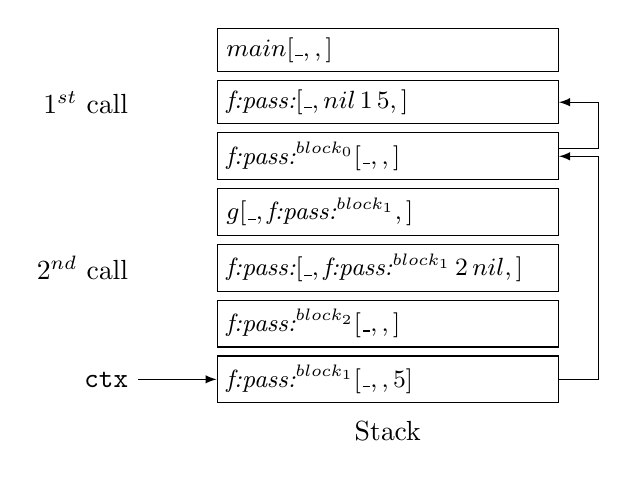
\begin{tikzpicture}[
block/.style={
draw,
fill=white,
rectangle, 
text width={4.1cm},
align=left,
font=\small}]
%  MainClass>>main[][], T>>f:pass:[nil, 1, 5][], T>>f:pass:-block0[][], T>>g:[f:pass:-block1][], T>>f:pass:[f:pass:-block1, 2, nil][], T>>f:pass:-block2[][], T>>f:pass:-block1[][5]

%listed with the top of the stack first, but drawn with top of the stack on the bottom
\node[block](a){$\text{\em f:pass:}^{block_1}[\_,,5]$};
\node[block,above=0.1cm of a](b){$\text{\em f:pass:}^{block_2}[\_,,]$};
\node[block,above=0.1cm of b](c){$\text{\em f:pass:}[\_,\text{\em f:pass:}^{block_1}\,2\,nil,]$};
\node[block,above=0.1cm of c](d){$g[\_,\text{\em f:pass:}^{block_1},]$};
\node[block,above=0.1cm of d](e){$\text{\em f:pass:}^{block_0}[\_,,]$};
\node[block,above=0.1cm of e](f){$\text{\em f:pass:}[\_,nil\,1\,5,]$};
\node[block,above=0.1cm of f](g){$main[\_,,]$};

\node[draw=none,,below=0.1cm of a]{Stack};
\draw[-latex] (a.east) -- ++(5mm,0) |- (e.east);
\draw[-latex] ($(e.east)+(0,.1)$) -- ++(5mm,0) |- ($(f.east)$);
\node[left=of f] {$1^{st}$ call};
\node[left=of c] {$2^{nd}$ call};
\node[left=of a](x) {{\tt ctx}};
\draw[-latex] (x.east) |- (a.west);
\end{tikzpicture}
\end{center}
{\em Notes}:  The enclosing block of {\tt [x:=5]} (called $\text{\em f:pass:}^{block_1}$) is {\tt [self g:[x:=5]]} (called $\text{\em f:pass:}^{block_0}$). The enclosing block of $\text{\em f:pass:}^{block_0}$ is the first call, not the second call, to $\text{\em f:pass:}$.
\end{minipage} \\
\end{tabular}

%------------CODE GEN---------------------

\def\arraystretch{1.0}

\begin{figure}
\begin{center}
\begin{tabular}[t]{r | l | l }
{\bf Smalltalk fragment} & {\bf Visitor method result} & {\bf Side-effects}\\
\hline
$\epsilon$ & $\epsilon$ (object {\tt Code.None}) & \\

{\tt class T : S [ ]} & $\epsilon$ & \\

$main$  & 
\begin{minipage}[t]{0.25\linewidth}
$main$\\
{\tt self\\
return}\vspace{5pt}
\end{minipage} & \\

{\tt f <primitive:\#}{\it primitive-name}{\tt >} &
\begin{minipage}[t]{0.35\linewidth}
$\epsilon$ \vspace{7pt}
\end{minipage} &  \\

{\tt f [ } {\tt ]} & $\epsilon$&
\begin{minipage}[t]{0.35\linewidth}
$\text{\tt f}_{\text{\it code}} =$ \\
\parbox{20pt}{~}{\tt self}\\
\parbox{20pt}{~}{\tt return}
\end{minipage} \\

{\tt f [ }$body$ {\tt ]} & $\epsilon$&
\begin{minipage}[t]{0.35\linewidth}
$\text{\tt f}_{\text{\it code}} =$ \\
\parbox{20pt}{~}$body$\\
\parbox{20pt}{~}{\tt pop}\\
\parbox{20pt}{~}{\tt self}\\
\parbox{20pt}{~}{\tt return}
\end{minipage} \\

{\it operator} {\tt [ }{\it body} {\tt ]} & $\epsilon$&
\begin{minipage}[t]{0.35\linewidth}
$\text{\it operator}_{\text{\it code}} =$ \\
\parbox{20pt}{~}$body$\\
\parbox{20pt}{~}{\tt pop}\\
\parbox{20pt}{~}{\tt self}\\
\parbox{20pt}{~}{\tt return}
\end{minipage} \\

{\tt a:\,x b:\,y c:\,z [ }{\it body} {\tt ]}  & $\epsilon$&
\begin{minipage}[t]{0.35\linewidth}
$\text{\tt a:b:c:}_{\text{\it code}} =$ \\
\parbox{20pt}{~}$body$\\
\parbox{20pt}{~}{\tt pop}\\
\parbox{20pt}{~}{\tt self}\\
\parbox{20pt}{~}{\tt return}
\end{minipage} \\

$\underbrace{\text{\tt [$args$| |$locals$|  ]}}_{\text{\tt f}^{block_i}}$ & {\tt block }$i$ &
\begin{minipage}[t]{0.35\linewidth}
$\text{\tt f}_{block_i} =$\\
\parbox{20pt}{~}{\tt nil \\
\parbox{20pt}{~}block\_return}
\end{minipage} \\

$\underbrace{\text{\tt [ $body$ ]}}_{\text{\tt f}^{block_i}}$ & {\tt block }$i$ &
\begin{minipage}[t]{0.35\linewidth}
$\text{\tt f}_{block_i}=$\\
\parbox{20pt}{~}$body$\\
\parbox{20pt}{~}{\tt block\_return}
\end{minipage} \\

{\tt $expr_1.\, expr_2. \,\cdots\, expr_n$} &
\begin{minipage}[t]{0.25\linewidth}
$expr_1$\\
{\tt pop}\\
$expr_2$\\
{\tt pop}\\
$\cdots$\\
$expr_n$\vspace{5pt}
\end{minipage} 
& \\

\end{tabular}
\end{center}
\vspace{-10pt}
\caption{Smalltalk Class/Method/Block Compilation Rules}
\label{default}
\end{figure}%

%------------EXPRESSION GEN---------------------

\def\arraystretch{1.0}

\begin{figure}
\begin{center}
\begin{tabular}[t]{r | l | l }
{\bf Smalltalk fragment} & {\bf Visitor method result} & {\bf Side-effects}\\
\hline
${\tt class~ T~[|}x_0 x_1 ..\, x_n|\cdots {\tt f} \,[\, \cdots~ x_i {\tt :=} \,expr$ &
\begin{minipage}[t]{0.25\linewidth}
$expr$\\
{\tt store\_field} $i$\vspace{5pt}
\end{minipage} & \\

$\text{\tt a:}x_0 \,\,\text{\tt b:}x_1~{\tt [|}x_2 ..\, x_n |\cdots~ x_i {\tt :=} \,expr$ &
\begin{minipage}[t]{0.25\linewidth}
$expr$\\
{\tt store\_local} $0, i$\vspace{3pt}
\end{minipage} & \\

${\tt f~[|}x_0 ..\, x_n| \cdots~ x_i {\tt :=} \,expr$ &
\begin{minipage}[t]{0.25\linewidth}
$expr$\\
{\tt store\_local} $0, i$\vspace{3pt}
\end{minipage} & \\

${\tt f~[\, \cdots~ [|}x_0 ..\, x_n| \cdots~ x_i {\tt :=} \,expr$ &
\begin{minipage}[t]{0.25\linewidth}
$expr$\\
{\tt store\_local} $0, i$\vspace{3pt}
\end{minipage} & \\

$\underbrace{\text{\tt f:}{\tt x~}{\tt [}\cdots [}_{\Delta \,=\,\#scopes} \cdots\, \text{\tt x} {\tt :=}\, expr$ &
\begin{minipage}[t]{0.25\linewidth}
{\tt store\_local} $\Delta, 0$
\end{minipage} & \\

$\text{\tt f [}\cdots\underbrace{{\tt [|x| }\cdots [}_{\Delta}\cdots~ \text{\tt x} {\tt :=} \,expr$ &
\begin{minipage}[t]{0.25\linewidth}
$expr$\\
{\tt store\_local} $\Delta, 0$\vspace{5pt}
\end{minipage} & \\

${\tt class~ T~[|}x_0 x_1 ..\, x_n|\cdots {\tt f}\, [\, \cdots~ x_i$ & 
\begin{minipage}[t]{0.25\linewidth}
{\tt push\_field} $i$ \vspace{5pt}
\end{minipage} & \\

$\text{\tt a:}x_0 \,\,\text{\tt b:}x_1~{\tt [|}x_2 ..\, x_n |\cdots~ x_i$ &
\begin{minipage}[t]{0.25\linewidth}
{\tt push\_local} $0, i$\vspace{5pt}
\end{minipage} & \\

$\underbrace{\text{\tt f:}{\tt x~}{\tt [}\cdots [}_{\Delta \,=\,\#scopes} \cdots\, {\tt x}$ &
\begin{minipage}[t]{0.25\linewidth}
{\tt push\_local} $\Delta, 0$
\end{minipage} & \\

$\text{\tt f [}\cdots\underbrace{{\tt [|x| }\cdots [}_{\Delta}\cdots~ {\tt x}$ &
\begin{minipage}[t]{0.25\linewidth}
{\tt push\_local} $\Delta, 0$
\end{minipage} & \\

{\tt 99} & {\tt push\_int 99} & \\

{\tt \$a} & {\tt push\_char} {\em ASCII('a')}  & \\

{\tt 1.2} & {\tt push\_float} {\small\em asIntBits(1.2)} & \\

${\tt class~ T~[} \cdots\,$ {\tt 'a string'} & {\tt push\_literal} $i$ & $\text{\tt T}_{literal_i} = ``\text{\tt a string}$'' \\

{\tt nil} & {\tt nil} & \\

{\tt self} & {\tt self} & \\

{\tt true} & {\tt true} & \\

{\tt false} & {\tt false} & \\

\{ $expr_1.\, expr_2. \,\cdots\, expr_n$ \} &
\begin{minipage}[t]{0.2\linewidth}
$expr_1$\\
$expr_2$\\
$\cdots$\\
$expr_n$\\
{\tt push\_array} $n$
\end{minipage} & \\

\end{tabular}
\end{center}
\vspace{-10pt}
\caption{Smalltalk Expression Compilation Rules}
\label{default}
\end{figure}%

%------------MESSAGE EXPRESSION GEN---------------------

\def\arraystretch{1.0}

\begin{figure}
\begin{center}
\begin{tabular}[t]{r | l | l }
{\bf Smalltalk fragment} & {\bf Visitor results} & {\bf Side-effects}\\
\hline
(unary msg)~~~~~~~~~~~~\, ${\tt class~ T~[} \cdots\,$ {\tt f\,[}\,$\cdots ~expr \,w$ &
\begin{minipage}[t]{0.2\linewidth}
$expr$\\
{\tt send} $0,i$\vspace{5pt}
\end{minipage}  & $\text{\tt T}_{literal_i} = ``w$'' \\

(binary msg)~~~${\tt class~ T~[} \cdots\,$ {\tt f\,[}$\cdots ~expr_1\, op~ expr_2$ &
\begin{minipage}[t]{0.2\linewidth}
$expr_1$\\
$expr_2$\\
{\tt send} $1,i$\vspace{5pt}
\end{minipage}  & $\text{\tt T}_{literal_i} = ``op$'' \\

${\tt class~ T~[} \cdots\,$ {\tt f\,[}$\cdots ~expr ~w_1{\tt :} e_1 ~ w_2{\tt :} e_2 \, \cdots \, w_n{\tt :} e_n$ &
\begin{minipage}[t]{0.2\linewidth}
$expr$\\
$e_1$\\
$e_2$\\
$\cdots$\\
$e_n$\\
{\tt send} $n,i$\vspace{5pt}
\end{minipage}  & $\text{\tt T}_{literal_i} = ``w_1{\tt :}w_2{\tt :}\cdots w_n{\tt :}$'' \\

${\tt class~ T~[} \cdots\,$ {\tt f\,[}$\,\cdots \,{\tt super} \,w$ &
\begin{minipage}[t]{0.2\linewidth}
{\tt self}\\
{\tt send\_super} $0,i$\vspace{5pt}
\end{minipage}  & $\text{\tt T}_{literal_i} = ``w$'' \\

${\tt class~ T~[} \cdots\,$ {\tt f\,[}$\cdots ~{\tt super} ~w_1{\tt :} e_1 ~ w_2{\tt :} e_2 \, \cdots \, w_n{\tt :} e_n$ &
\begin{minipage}[t]{0.2\linewidth}
{\tt self}\\
$e_1$\\
$e_2$\\
$\cdots$\\
$e_n$\\
{\tt send\_super} $n,i$\vspace{3pt}
\end{minipage}  & $\text{\tt T}_{literal_i} = ``w_1{\tt :}w_2{\tt :}\cdots w_n{\tt :}$''\\

{\tt\Large \verb=^=}$expr$ &
\begin{minipage}[t]{0.2\linewidth}
$expr$\\
{\tt return}\vspace{5pt}
\end{minipage} & \\

\end{tabular}
\end{center}
\vspace{-10pt}
\caption{Smalltalk Message Expression Compilation Rules}
\label{default}
\end{figure}%

\begin{minipage}[t]{0.25\linewidth}
\end{minipage} 

\begin{minipage}[t]{0.25\linewidth}
\begin{alltt}
\end{alltt}
\end{minipage} 

\end{document}
